% !TEX TS-program = XeLaTeX
% use the following command:
% all document files must be coded in UTF-8
\documentclass[spanish]{textolivre}
% build HTML with: make4ht -e build.lua -c textolivre.cfg -x -u article "fn-in,svg,pic-align"

\journalname{Texto Livre}
\thevolume{15}
%\thenumber{1} % old template
\theyear{2022}
\receiveddate{\DTMdisplaydate{2021}{10}{31}{-1}} % YYYY MM DD
\accepteddate{\DTMdisplaydate{2022}{1}{11}{-1}}
\publisheddate{\DTMdisplaydate{2022}{1}{27}{-1}}
\corrauthor{Marta Magadán-Díaz}
\articledoi{10.35699/1983-3652.2022.36941}
%\articleid{NNNN} % if the article ID is not the last 5 numbers of its DOI, provide it using \articleid{} commmand
% list of available sesscions in the journal: articles, dossier, reports, essays, reviews, interviews
\articlesessionname{articles}
\runningauthor{Magadán-Díaz et al.} 
%\editorname{Leonardo Araújo} % old template
\sectioneditorname{Hugo Heredia Ponce}
\layouteditorname{Anna Izabella Pereira}

\title{Percepciones de los estudiantes de posgrado ante la gamificación del aula con Quizizz}
\othertitle{Percepções dos alunos de pós-graduação em face da gamificação em sala de aula com Quizizz}
\othertitle{Graduate students' perceptions of classroom gamification with Quizizz}
% if there is a third language title, add here:
%\othertitle{Artikelvorlage zur Einreichung beim Texto Livre Journal}

\author[1]{Marta Magadán-Díaz \orcid{0000-0003-3178-3215} \thanks{Email: \url{marta.magadan@unir.net}}}
\author[1]{Jesús I. Rivas-García \orcid{0000-0003-0576-5961} \thanks{Email: \url{jesus.rivas@unir.net}}}
\affil[1]{Universidad Internacional de La Rioja, Facultad de Empresa y Comunicación, La Rioja, España.}

\addbibresource{article.bib}
% use biber instead of bibtex
% $ biber article

% used to create dummy text for the template file
\definecolor{dark-gray}{gray}{0.35} % color used to display dummy texts
\usepackage{lipsum}
\SetLipsumParListSurrounders{\colorlet{oldcolor}{.}\color{dark-gray}}{\color{oldcolor}}

% used here only to provide the XeLaTeX and BibTeX logos
\usepackage{hologo}

% if you use multirows in a table, include the multirow package
\usepackage{multirow}

% provides sidewaysfigure environment
\usepackage{rotating}

% CUSTOM EPIGRAPH - BEGIN 
%%% https://tex.stackexchange.com/questions/193178/specific-epigraph-style
\usepackage{epigraph}
\renewcommand\textflush{flushright}
\makeatletter
\newlength\epitextskip
\pretocmd{\@epitext}{\em}{}{}
\apptocmd{\@epitext}{\em}{}{}
\patchcmd{\epigraph}{\@epitext{#1}\\}{\@epitext{#1}\\[\epitextskip]}{}{}
\makeatother
\setlength\epigraphrule{0pt}
\setlength\epitextskip{0.5ex}
\setlength\epigraphwidth{.7\textwidth}
% CUSTOM EPIGRAPH - END

% LANGUAGE - BEGIN
% ARABIC
% for languages that use special fonts, you must provide the typeface that will be used
% \setotherlanguage{arabic}
% \newfontfamily\arabicfont[Script=Arabic]{Amiri}
% \newfontfamily\arabicfontsf[Script=Arabic]{Amiri}
% \newfontfamily\arabicfonttt[Script=Arabic]{Amiri}
%
% in the article, to add arabic text use: \textlang{arabic}{ ... }
%
% RUSSIAN
% for russian text we also need to define fonts with support for Cyrillic script
% \usepackage{fontspec}
% \setotherlanguage{russian}
% \newfontfamily\cyrillicfont{Times New Roman}
% \newfontfamily\cyrillicfontsf{Times New Roman}[Script=Cyrillic]
% \newfontfamily\cyrillicfonttt{Times New Roman}[Script=Cyrillic]
%
% in the text use \begin{russian} ... \end{russian}
% LANGUAGE - END

% EMOJIS - BEGIN
% to use emoticons in your manuscript
% https://stackoverflow.com/questions/190145/how-to-insert-emoticons-in-latex/57076064
% using font Symbola, which has full support
% the font may be downloaded at:
% https://dn-works.com/ufas/
% add to preamble:
% \newfontfamily\Symbola{Symbola}
% in the text use:
% {\Symbola }
% EMOJIS - END

% LABEL REFERENCE TO DESCRIPTIVE LIST - BEGIN
% reference itens in a descriptive list using their labels instead of numbers
% insert the code below in the preambule:
%\makeatletter
%\let\orgdescriptionlabel\descriptionlabel
%\renewcommand*{\descriptionlabel}[1]{%
%  \let\orglabel\label
%  \let\label\@gobble
%  \phantomsection
%  \edef\@currentlabel{#1\unskip}%
%  \let\label\orglabel
%  \orgdescriptionlabel{#1}%
%}
%\makeatother
%
% in your document, use as illustraded here:
%\begin{description}
%  \item[first\label{itm1}] this is only an example;
%  % ...  add more items
%\end{description}
% LABEL REFERENCE TO DESCRIPTIVE LIST - END


% add line numbers for submission
%\usepackage{lineno}
%\linenumbers

% https://tex.stackexchange.com/questions/436052/unnecessary-white-space-between-words-in-latex-table
\usepackage{array,ragged2e}
\newcolumntype{P}[1]{>{\RaggedRight\arraybackslash}p{#1}}
%\newcolumntype{P}[1]{>{\RaggedRight\hspace{0pt}}p{#1}}

\begin{document}
\maketitle

\begin{polyabstract}
\begin{abstract}
El objetivo de esta investigación es examinar las percepciones que los discentes universitarios de posgrado tienen al utilizar Quizizz, en el contexto de la asignatura de Gestión Cultural Avanzada en el Ámbito Editorial, dentro del Máster Universitario en Gestión y Emprendimiento de Proyectos Culturales, en una universidad española de educación en línea. Para ello, se plantean las siguientes preguntas de investigación: a) ¿cuáles son las percepciones del alumnado sobre el uso de Quizizz en las clases de Gestión Cultural Avanzada en el Ámbito Editorial?; b) ¿qué variables identificadas en las entrevistas experimentan la mayoría de los estudiantes de posgrado que usan Quizizz en este contexto? y c) ¿los datos cuantitativos de la encuesta en línea validan los resultados de las entrevistas cualitativas iniciales? Se emplea una metodología mixta -cualitativa y cuantitativa- para dar respuesta a las cuestiones formuladas y se concluye que la percepción de los estudiantes de posgrado en relación con el uso de Quizizz en el aula virtual es positiva. Quizizz tiene un impacto positivo en la motivación, el compromiso y la dinamización del aula. Finalmente, el análisis cuantitativo confirma en buena medida el análisis cualitativo.

\keywords{Educación \sep Aprendizaje en línea \sep Innovación pedagógica \sep Actitud del estudiante \sep Juego educativo}
\end{abstract}

\begin{portuguese}
\begin{abstract}
O objetivo desta pesquisa é examinar as percepções que estudantes universitários de pós-graduação têm ao utilizar o Quizizz no contexto da disciplina de Gestão Cultural Avançada na Área Editorial, no âmbito do Mestrado em Gestão e Empreendedorismo de Projetos Culturais em uma universidade de Educação \textit{online} espanhola. Para isso, levantam-se as seguintes questões de pesquisa: a) qual a percepção dos alunos sobre a utilização do Quizizz nas aulas de Gestão Cultural Avançada na Área Editorial?; b) quais variáveis identificadas nas entrevistas a maioria dos alunos de pós-graduação que usam o Quizizz vivenciam nesse contexto? e c) os dados quantitativos da pesquisa \textit{online} validam os resultados das entrevistas qualitativas iniciais? Uma metodologia mista – qualitativa e quantitativa – é utilizada para responder às questões formuladas e conclui-se que a percepção dos alunos de pós-graduação em relação ao uso do Quizizz na sala de aula virtual é positiva. O Quizizz tem um impacto positivo na motivação, empenho e dinamização da sala de aula. Finalmente, a análise quantitativa confirma amplamente a análise qualitativa.

\keywords{Educação \sep Aprendizagem \textit{online} \sep Inovação pedagógica \sep Atitude do aluno \sep Jogo educativo}
\end{abstract}
\end{portuguese}

\begin{english}
\begin{abstract}
The objective of this research is to examine the perceptions that graduate university students have when using Quizizz, in the context of the subject of Advanced Cultural Management in the Publishing Field, within the Master's Degree in Management and Entrepreneurship of Cultural Projects at an online Spanish university. For this, this research poses the following questions: a) what are the students' perceptions about the use of Quizizz in the classes of Advanced Cultural Management in the Publishing Field ?; b) what variables identified in the interviews do most graduate students who use Quizizz experience in this context?, and c) does the quantitative data from the online survey validate the results of the initial qualitative interviews? A mixed methodology – qualitative and quantitative – is used to answer the questions formulated, and it is concluded that the perception of postgraduate students concerning the use of Quizizz in the virtual classroom is positive. Quizizz has a positive impact on the motivation, commitment, and dynamization of the virtual classroom. Finally, the quantitative analysis confirms the qualitative one.

\keywords{Education \sep Online learning  \sep Teaching method innovations \sep Student attitudes \sep Educational games}
\end{abstract}
\end{english}
% if there is another abstract, insert it here using the same scheme
\end{polyabstract}

\section{Introducción}\label{sec-intro}
Un sector clave en el que se está explorando activamente la gamificación, principalmente por su potencial para motivar, es la educación \cite{dichev2017}. La gamificación es una estrategia de aprendizaje que, mediante la incorporación de elementos del juego, aumenta el compromiso del estudiante con el objeto de conseguir mejores resultados académicos \cite{dichev2017, sanchez2020}. Los principales objetivos de la gamificación son: a) mejorar ciertas habilidades, b) introducir objetivos que den un propósito al aprendizaje, c) involucrar a los estudiantes, d) optimizar el aprendizaje, e) apoyar el cambio de comportamiento y socializar, f) intensificar la concentración de los discentes y g) mejorar su motivación para el trabajo en grupo \cite{dewi2021, dichev2017, licorish2018}.

Dada la idea de que los juegos en el aula resultan amenos y divertidos, muchos docentes han integrado la gamificación en sus clases y los investigadores han comenzado a analizar el impacto del uso de los juegos en el proceso de aprendizaje de los discentes \cite{mekler2017}. Aunque la gamificación en el aula no es un método nuevo, cuando se fusiona con la tecnología se convierte en un poderoso instrumento de enseñanza y aprendizaje para las generaciones acostumbradas a utilizar Internet \cite{bicen2018}. El uso generalizado de la tecnología móvil en el aula actual ha creado nuevas oportunidades para que los docentes adopten la gamificación digital en la enseñanza \cite{saleem2021}. Esta herramienta favorece: a) el proceso de enseñanza-aprendizaje, al elevar el nivel de compromiso del alumnado en el estudio de la asignatura; b) la resolución de pruebas de opción múltiple con un enfoque más optimista y autoconfianza; c) mayor predisposición de los estudiantes al trabajo en equipo; y d) un ambiente educativo entretenido y motivador \cite{vergara_rodriguez2019}.

Los sistemas de respuesta de los discentes basados en el juego (GSRS) proporcionan una experiencia de aprendizaje competitiva y amigable que, a su vez, crea una atmósfera agradable en el aula. La gamificación digital puede agregar un nivel adicional de motivación, compromiso e incentivo en muchas aulas \cite{doumanis2019, infante-villagran2021}. Los aspectos motivacionales involucrados en los GSRS incluyen competición, tablas de clasificación en desafíos, insignias por logros, puntos de recompensa y ciclos de retroalimentación instantánea, permitiendo a los estudiantes participar en el contenido educativo de manera lúdica y dinámica \cite{bottentuit2020, hanus2015}. Los contenidos educativos incorporados en una gamificación digital parecen hacer que el aprendizaje resulte más divertido y atractivo \cite{magadan-diaz2021}.

Quizizz es una aplicación educativa que aplica el concepto de gamificación \cite{pahamzah2020, zhao2019}. Es una herramienta de evaluación en línea que se puede descargar y utilizar de forma gratuita \cite{amalia2020}. Fue creada en 2015 por dos profesores indios que diseñaron el sistema teniendo en cuenta su experiencia en la enseñanza de matemáticas en una escuela de Bangalore (India). Hoy en día, Quizizz es utilizado por millones de profesores y estudiantes en más de 100 países \cite{andayani2021, bottentuit2020}. Quizizz permite agregar avatares, memes, música, límites de tiempo e imágenes con el propósito de motivar al alumnado para participar en el juego, competir entre ellos y estudiar para conseguir mejores resultados al jugar \cite{degirmenci2021, rahmawati2021, yunus2021, zuhriyah2020}.

El proceso para hacer uso de Quizizz es el siguiente: en primer lugar, entrar en la web (\url{https://quizizz.com}) y hacer click en comenzar (\emph{get started}); en segundo lugar, crear una cuenta con un correo electrónico, pudiendo elegir entre tres opciones de ingreso, como profesor (\emph{teacher}), estudiante (\emph{student}) o tutor o padre (\emph{parent or guardian}); en tercer lugar, completar la información solicitada para la portada como título, descripción e idioma; en cuarto lugar, crear las preguntas y respuestas, pudiéndose agregar imágenes e incluir de 1 a 5 opciones de respuesta; en quinto lugar, ajustar el tiempo; en sexto lugar, presionar el botón terminar (\emph{finish}) una vez completado el cuestionario y, finalmente, dar el código PIN o código de acceso a los estudiantes para poder ser utilizado \cite{bottentuit2020}.

El objetivo general de este estudio es examinar las percepciones que los discentes universitarios de posgrado tienen al utilizar Quizizz, en el contexto de la asignatura de Gestión Cultural Avanzada en el Ámbito Editorial, dentro del Máster Universitario en Gestión y Emprendimiento de Proyectos Culturales, en una universidad española de educación en línea. Para alcanzar el objetivo general de este trabajo, se plantean las siguientes preguntas de investigación:

\begin{itemize}
    \item[RQ1:] ¿Cuáles son las percepciones del alumnado sobre el uso de Quizizz en las clases de Gestión Cultural Avanzada en el Ámbito Editorial?
    \item[RQ2:] ¿Qué variables identificadas en las entrevistas experimentan la mayoría de los estudiantes de posgrado que usan Quizizz en este contexto? 
    \item[RQ3:] ¿Los datos cuantitativos de la encuesta en línea validan los resultados de las entrevistas cualitativas iniciales?
\end{itemize}

Este estudio se estructura del siguiente modo: la sección \ref{sec-2} aborda la revisión de la literatura; la sección \ref{sec-3} expone la metodología; la sección \ref{sec-4} recoge los resultados y finalmente la sección \ref{sec-5} destaca las conclusiones.

\section{Revisión de la literatura}\label{sec-2}
La literatura académica sobre los GSRS ha señalado que el proceso de aprendizaje resulta más divertido cuando los jugadores afrontan el desafío de tareas de resolución de problemas en un entorno audiovisual estimulante e identifica tres factores que influyen en la motivación intrínseca: el desafío, la fantasía y curiosidad \cite{licorish2018, malone1981, wang2015}. La curiosidad se traduce en la motivación de los estudiantes para aprender \cite{ryan2000}. La curiosidad se activa con la música, los colores, los efectos de audio, la retroalimentación instantánea y las habilidades interactivas que ofrecen los GSRS \cite{malone1981}. Los discentes encuentran emocionantes los juegos digitales porque los juegos crean una sensación de control y empoderamiento del usuario \cite{malone1981}. Cuando los jugadores tienen más control sobre su aprendizaje, experimentan una intensa concentración y emoción. El alumnado a implicarse más en el aprendizaje a medida que con la gamificación obtienen más puntos, alcanzan niveles más altos en el juego y superan a otros competidores individualmente o en equipo \cite{dominguez2013, malone1987}.

Las interacciones con el entorno social, incluidos los compañeros, son necesarias para facilitar el crecimiento cognitivo del alumno, mejorar la comprensión, desarrollar el pensamiento crítico y mejorar el aprendizaje de orden superior \cite{pahamzah2020}. De manera similar, la gamificación que se encuentra en los GSRS puede promover un aprendizaje efectivo, ya que brinda a los alumnos la oportunidad de practicar y reflexionar en un contexto basado en problemas \cite{awwal2015}. Los alumnos deben sentirse desafiados pero tal desafío debe ubicarse dentro de la zona de desarrollo próximo (ZDP) para sentirse competentes al afrontarlo \cite{vygotskii1978}. Los GSRS alientan a los estudiantes con desafíos que se encuentran en su ZDP además de facilitar la interacción social enriquecedora \cite{chaiklin2003}.

Diversos autores han relacionado el uso de los GSRS en el aula con los resultados educativos positivos de los discentes. En particular, se ha encontrado que los GSRS generan una motivación positiva de los estudiantes por aprender \cite{iaremenko2017}, promueven la participación \cite{bottentuit2020, wang2015}, facilitan las discusiones en el aula \cite{mason2021} y mejoran los resultados del aprendizaje \cite{dakka2015}. Además, se ha descubierto que mejoran la dinámica del aula \cite{hung2017, yunus2021}, aumentan la interacción instructor-alumno \cite{mendez2013}, reducen las distracciones \cite{licorish2018} y facilitan la evaluación formativa \cite{balta2018, dewi2021}. En resumen, los GSRS se consideran beneficiosos al aumentar el compromiso, la motivación, la percepción de aprendizaje y la dinámica del aula \cite{fakhruddin2020}.

El uso de los GSRS transmite una serie de beneficios al proceso docente \cite{wentao2017}. Se ha descubierto que estas tecnologías interactivas aumentan la asistencia, mejoran la capacidad de atención, promueven la discusión en el aula, hacen que las conferencias sean más divertidas, mejoran la interacción en el aula, favorecen la participación anónima y brindan a los estudiantes oportunidades para la reflexión \cite{goksun2019, wang2015}.

Se ha observado que los discentes creen que Quizizz es una herramienta divertida y atractiva \cite{zuhriyah2020}. Los hallazgos mostraron que los estudiantes tienen una buena percepción de la implementación de Quizizz en el aprendizaje \cite{dewi2021}. Además, Quizizz puede impulsar su confianza en sí mismos para motivar al alumnado y aumentar su capacidad para aprender \cite{irwansyah2021, zuhriyah2020}. La investigación encontró que los discentes piensan que Quizizz es más efectivo que Kahoot \cite{goksun2019}. Los GSRS, como Quizizz, ayudan también al alumnado a mejorar el desarrollo de sus competencias \cite{sahak2021, wolff2016} y su experiencia de aprendizaje \cite{chaiyo2017}. Hay estudios que indican que aquellos docentes que aplicaron Quizizz obtuvieron de sus discentes puntuaciones más altas en la evaluación del desempeño docente \cite{zhao2019}.

A pesar de las percepciones generalmente positivas de los GSRS, la literatura académica también se ha encontrado con algunos inconvenientes que incluyen: desafíos técnicos, redes inalámbricas poco confiables e ineficacia académica \cite{aljaloud2015}. La participación anónima puede aumentar las conjeturas a ciegas, lo que no siempre refleja con precisión el nivel de comprensión de los estudiantes \cite{nielsen2013}. El uso repetido e intenso en el aula de GSRS puede conducir a un cierto aburrimiento entre el alumnado derivado de un efecto desgaste de la dinámica del aula que pasa de novedosa a rutinaria \cite{wang2015}. Los alumnos pueden ver los cuestionarios y los ejercicios realizados a través de Quizizz como tareas aburridas \cite{mohamad2020}. El aparecer clasificado entre los discentes con puntuaciones más bajas parece desmotivar más que motivar, impactando negativamente en la participación \cite{bottentuit2020}. Otro factor que parece influir negativamente en la experiencia de los estudiantes con los GSRS es el relativo a las interrupciones en el aula causadas por la intensa emoción experimentada por el alumnado mientras juegan \cite{mason2021}.

\section{Metodología}\label{sec-3}
Esta investigación emplea una metodología mixta, cualitativa y cuantitativa y el diseño exploratorio empleado fue un diseño secuencial, donde el componente central es cualitativo y el componente complementario es cuantitativo, es decir, un enfoque QUAL→quan. Este diseño secuencial exploratorio se caracteriza por dos fases de recopilación de datos (ver \Cref{fig1}) \cite{schoonenboom2017}.

\begin{figure}[htbp]
 \centering
 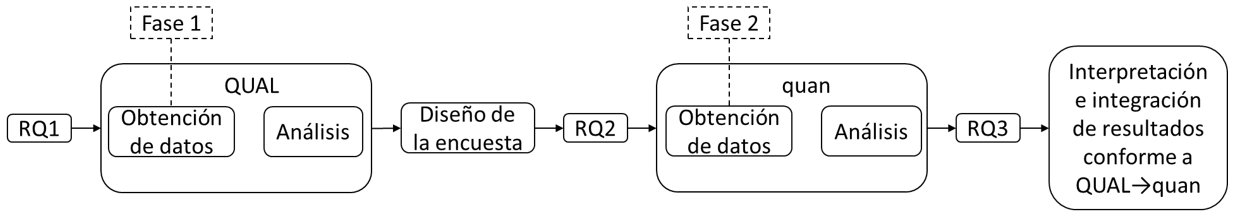
\includegraphics[width=\textwidth]{36941-fig1.png}
 \caption{Diseño secuencial exploratorio QUAL → quan}
 \label{fig1}
 \source{elaboración propia.‬‬‬‬‬‬‬‬‬‬‬‬‬‬‬}
\end{figure}

Los participantes fueron 106 estudiantes de la asignatura Gestión Cultural Avanzada en el Ámbito Editorial en el Máster Universitario en Gestión y Emprendimiento de Proyectos Culturales. El estudio fue diseñado siguiendo los principios éticos de la Declaración de Helsinki. Antes de su participación, los participantes fueron informados sobre los objetivos del estudio y sobre las pautas éticas seguidas en el diseño y tratamiento de los datos. La selección se realizó mediante un muestreo no probabilístico por conveniencia. Los datos sociodemográficos de los participantes se resumen en la \Cref{tab1}.

\begin{table}[htpb]
\caption{Perfil sociodemográfico de los participantes.}
\label{tab1}
\centering
\begin{tabular}{lll}
\toprule 
Características	& Frecuencia (n) & Porcentaje (\%)
\\ 
\midrule
\multicolumn{3}{c}{Edad}
\\ 
\arrayrulecolor[gray]{.7}
\midrule
\arrayrulecolor{black}
21-25 & 2 & 1,9
\\
26-30 & 14 & 13,2
\\
31-35 & 28 & 26,4
\\
36-40 & 45 & 42,5
\\
>40 & 17 & 16
\\
\midrule
\multicolumn{3}{c}{Género}
\\
\arrayrulecolor[gray]{.7}
\midrule
\arrayrulecolor{black}
Mujer & 52 & 49
\\
Hombre & 54 & 51
\\
\midrule
\multicolumn{3}{c}{País de origen}
\\
\arrayrulecolor[gray]{.7}
\midrule
\arrayrulecolor{black}
España & 51 & 48,1
\\
Colombia & 17 & 16
\\
Ecuador & 38 & 35,9
\\
\midrule
\multicolumn{3}{c}{Formación previa}
\\
\arrayrulecolor[gray]{.7}
\midrule
\arrayrulecolor{black}
Formación socioeconómica & 62 & 58,5
\\
Otra formación & 44 & 41,5
\\
\midrule
\multicolumn{3}{c}{Profesional/Trabajador en activo}
\\
\arrayrulecolor[gray]{.7}
\midrule
\arrayrulecolor{black}
Sí & 91 & 85,8
\\
No & 15 & 14,2
\\
\midrule
\multicolumn{3}{c}{Experiencia previa en formación online}
\\
\arrayrulecolor[gray]{.7}
\midrule
\arrayrulecolor{black}
Sí & 6 & 5,7
\\
No & 100 & 94,3
\\ 
\bottomrule
\end{tabular}
\source{elaboración propia.}
\end{table}

Los cuestionarios de opción múltiple de Quizizz fueron diseñados por los autores de esta investigación. Los estudiantes que asistían al aula virtual recibían el código de acceso o PIN para comenzar su dinámica de juego. Estas dinámicas se desarrollaron en semanas alternas -una sesión con Quizizz cada dos semanas- durante un cuatrimestre académico en dos promociones, 2019-20 y 2020-21. Las actividades se diseñaron para ser realizadas en un intervalo de tiempo comprendido entre los 15 y 20 minutos. Cada cuestionario contenía entre 20 y 30 preguntas cerradas de diverso tipo: opción múltiple, verdadero/falso o completar parte de frases relacionadas con conceptos técnicos, entre otras. Dos semanas antes de la finalización de la asignatura, se empleó Quizizz para reforzar el entrenamiento de los discentes de cara al examen final.

Durante el análisis cualitativo de datos, se siguieron estos pasos. Primero, se revisaron los comentarios de los estudiantes, se destacaron las frases clave y se interpretaron los datos para generalizar los códigos. Estos códigos se utilizaron para etiquetar y capturar algo interesante en los datos. A continuación, este proceso dio como resultado 10 códigos, que se emparejaron y organizaron para generar temas potenciales. Luego, los temas principales fueron revisados y organizados en 5 categorías (Tabla 2). Finalmente, se produjeron elementos para la encuesta.

\begin{table}[htpb]
\caption{Temas surgidos del análisis cualititativo de las entrevistas.}
\label{tab2}
\centering
\begin{tabular}{p{0.35\textwidth}p{0.35\textwidth}}
\toprule 
Tema & Área de contenido
\\ 
\midrule
Diversión & \multirow{2}{=}{Diversión y placer}
\\
Placer &
\\
Motivación & \multirow{2}{=}{Motivación y competitividad}
\\
Competitividad & 
\\
Interacción & \multirow{2}{=}{Interacción y compromiso}
\\
Compromiso	&
\\
Atención & \multirow{2}{=}{Atención y enfoque}
\\
Enfoque	& 
\\
Aprendizaje & \multirow{2}{=}{Aprendizaje y asimilación del conocimiento}
\\
Asimilación del conocimiento	
\\ 
\bottomrule
\end{tabular}
\source{elaboración propia.}
\end{table}

Para abordar el análisis cuantitativo, esta investigación hizo uso del método de encuesta online a través de la herramienta Google Forms para identificar qué variables se experimentaron en mayor medida por los estudiantes. La primera parte de la encuesta incluyó el propósito del estudio y preguntas generales para identificar la información sociodemográfica del participante (ver \Cref{tab1}). La segunda parte de la encuesta contenía 16 cuestiones usando una escala Likert (ver \Cref{tab3}) que van de 1 a 5 y cuyos valores tienen los siguientes significados: 5, totalmente de acuerdo; 4, de acuerdo; 3, no estoy seguro; 2, en desacuerdo y 1, totalmente en desacuerdo. Las 16 cuestiones están distribuidas en cinco categorías: atención y enfoque (3), interacción y compromiso (3), motivación y competencia (4), aprendizaje y retención de conocimientos (3) diversión y disfrute (3). 

\setlength\LTleft{-1in}
\setlength\LTright{-1in}
\begin{small}
\renewcommand{\arraystretch}{1.5}
\begin{longtable}{
    >{\raggedright\arraybackslash}p{0.4\textwidth}
    P{0.12\textwidth}
    P{0.12\textwidth}
    P{0.12\textwidth}
    P{0.12\textwidth}
    P{0.12\textwidth}}
\caption{Cuestiones.}
\label{tab3}
\\
\toprule
\multicolumn{6}{c}{Interacción y compromiso}
\\
\midrule
1. No tengo ganas de interactuar con el material cuando uso Quizizz. & Muy de acuerdo (5) & De acuerdo (4) & No seguro (3) & En desacuerdo (2) & Muy en desacuerdo (1)
\\
2. Siento que Quizizz hace la sesión virtual más interactiva y dinámica. & Muy de acuerdo (5) & De acuerdo (4) & No seguro (3) & En desacuerdo (2) & Muy en desacuerdo (1)
\\
3. Estuve comprometido y entusiasmado mientras jugaba con Quizizz. & Muy de acuerdo (5) & De acuerdo (4) & No seguro (3) & En desacuerdo (2) & Muy en desacuerdo (1)
\\
\midrule
\multicolumn{6}{c}{Atención y enfoque}
\\
\midrule
4. Me concentro más mientras juego con Quizizz para obtener una buena clasificación. & Muy de acuerdo (5) & De acuerdo (4) & No seguro (3) & En desacuerdo (2) & Muy en desacuerdo (1)
\\
5. Quizizz me ayuda a concentrarme. & Muy de acuerdo (5) & De acuerdo (4) & No seguro (3) & En desacuerdo (2) & Muy en desacuerdo (1)
\\
6. Me distraigo mientras juego con Quizizz. & Muy de acuerdo (5) & De acuerdo (4) & No seguro (3) & En desacuerdo (2) & Muy en desacuerdo (1)
\\
\midrule
\multicolumn{6}{c}{Motivación y competitividad}
\\
\midrule
7. El poder usar un apodo me motiva para jugar con Quizizz. & Muy de acuerdo (5) & De acuerdo (4) & No seguro (3) & En desacuerdo (2) & Muy en desacuerdo (1)
\\
8. Es importante para mí jugar bien con Quizizz para obtener buenos resultados. & Muy de acuerdo (5) & De acuerdo (4) & No seguro (3) & En desacuerdo (2) & Muy en desacuerdo (1)
\\
9. Trato de ganar al jugar con Quizizz. & Muy de acuerdo (5) & De acuerdo (4) & No seguro (3) & En desacuerdo (2) & Muy en desacuerdo (1)
\\
10. Resulta muy divertido competir con otras/os compañeras/os del aula virtual. & Muy de acuerdo (5) & De acuerdo (4) & No seguro (3) & En desacuerdo (2) & Muy en desacuerdo (1)
\\
\midrule
\multicolumn{6}{c}{Aprendizaje y asimilación del conocimiento}
\\
\midrule
11. Jugar con Quizizz me ayudó a comprender mejor los conceptos e ideas clave de la asignatura. & Muy de acuerdo (5) & De acuerdo (4) & No seguro (3) & En desacuerdo (2) & Muy en desacuerdo (1)
\\
12. A menudo comparto con mis compañeras/os mis argumentos para acertar con las respuestas correctas en Quizizz	& Muy de acuerdo (5) & De acuerdo (4) & No seguro (3) & En desacuerdo (2) & Muy en desacuerdo (1)
\\
13. Pienso que Quizizz no favorece una mejor experiencia de aprendizaje. & Muy de acuerdo (5) & De acuerdo (4) & No seguro (3)	& En desacuerdo (2) & Muy en desacuerdo (1)
\\
\midrule
\multicolumn{6}{c}{Diversión y disfrute}
\\
\midrule
14. Es divertido jugar con Quizizz. & Muy de acuerdo (5) & De acuerdo (4) & No seguro (3) & En desacuerdo (2) & Muy en desacuerdo (1)
\\
15. Es aburrido jugar con Quizizz. & Muy de acuerdo (5) & De acuerdo (4) & No seguro (3) & En desacuerdo (2) & Muy en desacuerdo (1)
\\
16. Me produce satisfacción ver mi nombre en el ranking de los mejores jugadores de Quizizz. & Muy de acuerdo (5) & De acuerdo (4) & No seguro (3) & En desacuerdo (2) & Muy en desacuerdo (1)
\\
\bottomrule
\source{elaboración propia.}
\end{longtable}
\end{small}

Antes de lanzar la encuesta, se hizo un control previo con un grupo reducido de alumnos fuera de la muestra. Gracias a dicho control se detectaron y corrigieron errores ortográficos y se reformularon aquellas partes de la encuesta cuya redacción resultase poco clara o ambiguas \cite{gideon2012}. Los análisis de datos estadísticos se realizaron con SPSS 25. El cuestionario fue previamente enviado a un grupo de académicos expertos, obteniéndose un valor alfa de Cronbach de $\alpha = 0.85$, mostrando una buena fiabilidad en la consistencia interna de la escala de medida.

Finalmente, es importante integrar y conectar los datos obtenidos por métodos cualitativos y cuantitativos para poder comprender los resultados obtenidos. La integración se define como la combinación de datos cualitativos y cuantitativos dentro de una etapa determinada de la investigación o dentro del propio análisis de datos \cite{akerblad2021}. En este estudio, la integración se produjo en la fase de diseño y desarrollo de la encuesta (guiada por el análisis cualitativo previo) y en la fase de resultados.

\section{Resultados}\label{sec-4}
Esta sección presenta una discusión de los hallazgos clave de las fases cualitativa y cuantitativa organizada en tres partes. La primera parte presenta los principales hallazgos y análisis de los datos cualitativos. La segunda parte informa los hallazgos cuantitativos y el análisis de la encuesta en línea. La tercera parte integra y analiza los hallazgos de ambas fases.

Las entrevistas semiestructuradas revelaron 5 pares de temas relacionados con la percepción del alumnado sobre Quizizz, que se presentan en las siguientes áreas: (1) atención y enfoque, (2) interacción y compromiso, (3) motivación y competencia, (4) aprendizaje y retención de conocimientos, y finalmente (5) diversión y disfrute.

El análisis de las entrevistas semiestructuradas reveló que todos los participantes parecen estar de acuerdo en que las sesiones semanales de Quizizz mantuvieron su atención. Los estudiantes creían que Quizizz les resultó útil para "recordar" y "memorizar información", mientras que algunos discentes destacaron que participar en los cuestionarios de Quizizz, especialmente antes del examen final, les ayudó mantenerse concentrados y refrescar la memoria \cite{licorish2018, vygotskii1978}.

Gran parte del alumnado afirmó que los efectos de sonido encontrados en Quizizz mantuvieron su compromiso y concentración \cite{malone1981, yunus2021}. Contrariamente a lo que se esperaría, el estudiante 6 declaró que los efectos de audio afectaron negativamente su concentración y se sintió distraída por la música y la presión del tiempo.

Una barrera importante para la concentración fue la duración de la lección, así como la hora del día en que se llevó a cabo. Los estudiantes detallaron que Quizizz alivió la sensación de fatiga y les dio un "descanso refrescante" de la sesión de 90 minutos. El estudiante 8 se refirió a su experiencia con Quizizz como una oportunidad para "recargarse" y "reenfocarse" cuando se sentía cansada en la última hora de la jornada académica.

Al igual que en estudios anteriores, el análisis de datos cualitativos mostró que Quizizz aumentó las oportunidades del alumnado para interactuar con sus compañeros y facilitó el compromiso profundo de los discentes con los materiales de contenido \cite{awedh2014, hung2017, mendez2013, wang2015}. Todos los participantes afirmaron que Quizizz fomentó la participación en el aula virtual y mejoró sus habilidades de colaboración.

Estos comentarios muestran elementos de aprendizaje activo \cite{dakka2015}. Además, los discentes informaron que tanto la participación en el aula virtual como la discusión con sus compañeros los mantuvieron concentrados. Además, algunos estudiantes sugirieron que Quizizz fue particularmente útil para cambiar la dinámica de la lección, ya que parecían sentir que formaban parte activa del proceso docente en lugar de ser meramente sujetos pasivos del proceso docente.

Otro punto clave que surgió de los datos fue el papel del anonimato en el aumento de la participación de los estudiantes. Si bien el anonimato en la participación a menudo se ve como un aspecto negativo de los GSRS \cite{nielsen2013}, permitir que los discentes usen apodos parece fomentar una participación más amplia. Durante las entrevistas, algunos expresaron que se sentían más cómodos al usar apodos porque les preocupaba elegir las respuestas incorrectas. Además, pensaron que usar apodos era realmente divertido, mientras que otros confirmaron que usaron apodos solo si no se sentían preparados para obtener buenos resultados en el juego \cite{bottentuit2020, licorish2018}.

Los estudiantes también apreciaron la competencia que experimentaron mientras participaban en Quizizz, incluido el uso de puntos, tabla de clasificación, presión de tiempo, estado, música de suspenso y rangos, que parece mantener su compromiso.

Parece que Quizizz fue visto por los discentes como una excusa para romper el hielo, animándolos a interactuar más con sus compañeros de aula virtual. En general, los comentarios de los participantes sugirieron una satisfacción general en términos de interacción, compromiso y colaboración con los compañeros.

Los datos cualitativos mostraron que todos los estudiantes ($n = 9$) creían que Quizizz fomentaba una competencia amistosa en el aula virtual, lo que mejoraba su motivación para aprender. Estos hallazgos parecen sugerir que Quizizz es intrínsecamente motivador porque satisface el deseo del alumnado por el desafío, la curiosidad y la fantasía \cite{malone1981}. Un estudiante comentó que la clasificación hizo que el cuestionario fuera más emocionante, mientras que otro estudiante enfatizó que era importante para él "esforzarse más" y estudiar para ganar el juego \cite{iaremenko2017}.

Algunos estudiantes estuvieron de acuerdo en que se concentraron más cuando competían entre sí, mientras que otros confirmaron que estudiaron antes de la clase para ganar. Este resultado respalda los efectos previamente documentados de los GSRS sobre la motivación y el compromiso \cite{grinias2017, malone1981, wang2020}: la intensa excitación motivada por la competencia y el control son factores clave para mantener la motivación intrínseca.

En cuanto a la variable de aprendizaje, el análisis cualitativo mostró que los estudiantes percibieron que Quizizz les ayudó a mejorar su desempeño en el aprendizaje. De los once discentes entrevistados, cinco expresaron que esta plataforma tuvo un impacto positivo en su rendimiento, y los demás reconocieron que las pruebas con Quizizz les ayudaron a repasar para el examen final.

Los estudiantes confirmaron que Quizizz les ayudó a recordar información previa y ayudarles a comprender el tema \cite{sahak2021, wolff2016}. También enfatizaron dos resultados de aprendizaje: la retención de conocimientos y la identificación de dificultades de aprendizaje. Varios discentes describieron a Quizizz como una herramienta útil para reforzar sus conocimientos, y algunos percibieron que Quizizz les había ayudado a identificar sus errores y aprender las respuestas correctas.

Además, parece que Quizizz mejoró la comprensión conceptual de los estudiantes debido al uso de imágenes, gráficos y comentarios instantáneos. El alumnado encontró una retroalimentación oportuna muy útil sobre su progreso. Algunos indicaron que las sesiones de Quizizz proporcionaron orientación para el aprendizaje y oportunidades para la autoevaluación \cite{dewi2021, mason2021}.

Muchos estudiantes percibieron el impacto en su rendimiento como un beneficio distintivo de Quizizz. Notaron que jugar con Quizizz les ayudó a prepararse para los exámenes y, en consecuencia, su estudio estaba más enfocado \cite{balta2018, mason2021}. Curiosamente, solo un estudiante no percibió que Quizizz le ayudara a mejorar los resultados de sus exámenes finales, lo que concuerda con el trabajo de \cite{vergara_rodriguez2019}.

Entre las variables, la motivación intrínseca de la diversión y el disfrute prevalece como una de las más experimentadas por los estudiantes de posgrado en el uso de Quizizz. El análisis de datos cualitativos mostró que todos estuvieron de acuerdo en que el elemento de diversión que se encuentra en el GSRS contribuye a una experiencia de clase más positiva. También percibieron los cuestionarios de Quizizz como satisfactorios y gratificantes. Los discentes sugirieron que Quizizz puede disminuir el aburrimiento, hacer que el tiempo de clase sea más divertido y reducir las distracciones causadas por los teléfonos móviles.

Los estudiantes también encontraron que Quizizz era fácil de usar. Parece que las tablas de clasificación les ofrecieron la oportunidad de ser reconocidos, lo que tal vez no hubiera sido posible con el uso de los entornos tradicionales en el aula virtual. Algunos expresaron que la clasificación obtenida mientras jugaban Quizizz agregó un elemento de alegría y les dio la oportunidad de enorgullecerse de sus logros, lo que impulsó su autoestima.

Algunos estudiantes manifestaron que las clases eran particularmente interesantes con el uso de Quizizz, mientras que varios describieron las sesiones en el aula virtual como divertidas y emocionantes \cite{bottentuit2020, licorish2018, yunus2021}.

La distribución de las respuestas obtenidas en la encuesta según los temas y cuestiones planteadas se muestra en la \Cref{tab4}.

\setlength\LTleft{-1in}
\setlength\LTright{-1in}
\begin{small}
\renewcommand{\arraystretch}{1.5}
\begin{longtable}{
    >{\raggedright\arraybackslash}p{0.3\textwidth}
    p{0.15\textwidth}
    p{0.13\textwidth}
    p{0.12\textwidth}
    p{0.15\textwidth}
    p{0.16\textwidth}}
\caption{Encuesta y distribución de las respuestas obtenidas según la escala de Likert.}
\label{tab4}
\\
\toprule
n=106 & Muy de acuerdo (5) & De acuerdo (4) & No seguro (3) & En desacuerdo (2) & Muy en desacuerdo (1)
\\
\midrule
\multicolumn{6}{c}{Interacción y compromiso}
\\
\arrayrulecolor[gray]{.7}
\midrule
\arrayrulecolor{black}
1. No tengo ganas de interactuar con el material cuando uso Quizizz. & 51 (48.1\%) & 5 (4.7\%) & 10 (9.4\%) & 8 (7.6\%) & 32 (30.2\%)
\\
2. Siento que Quizizz hace la sesión virtual más interactiva y dinámica. & 64 (60.4\%) & 12 (11.3\%) & 4 (3.8\%) & 7 (6.6\%) & 19 (17.9\%)
\\
\endfirsthead
3. Estuve comprometido y entusiasmado mientras jugaba con Quizizz. & 56 (52.8\%) & 15 (14.2\%) & 10 (9.4\%) & 7 (6.6\%) & 18 (17.0\%)
\\
\midrule
\multicolumn{6}{c}{Atención y enfoque}
\\
\arrayrulecolor[gray]{.7}
\midrule
\arrayrulecolor{black}
4. Me concentro más mientras juego con Quizizz para obtener una buena clasificación. & 63 (59.4\%) & 18 (17.0\%) & 8 (7.6\%) & 5 (4.7\%) & 12 (11.3\%)
\\
5. Quizizz me ayuda a concentrarme.	& 59 (55.7\%) & 17 (16.0\%) & 10 (9.4\%) & 7 (6.6\%) & 13 (12.3\%)
\\
6. Me distraigo mientras juego con Quizizz. & 46 (43.3\%) & 13 (12.3\%) & 14 (13.2\%) & 11 (10.4\%) & 22 (20.8\%)
\\
\midrule
\multicolumn{6}{c}{Motivación y competitividad}
\\
\arrayrulecolor[gray]{.7}
\midrule
\arrayrulecolor{black}
7. El poder usar un apodo me motiva para jugar con Quizizz. & 32 (30.1\%) & 13 (12.3\%) & 26 (24.5\%) & 11 (10.4\%) & 24 (22.7\%)
\\
8. Es importante para mí jugar bien con Quizizz para obtener buenos resultados. & 58 (54.7\%) & 16 (15.1\%) & 19 (18.0\%) & 4 (3.8\%) & 9 (8.4\%)
\\
9. Trato de ganar al jugar con Quizizz. & 52 (49.0\%) & 12 (11.3\%) & 13 (12.3\%)	& 11 (10.4\%) & 18 (17.0\%)
\\
10. Resulta muy divertido competir con otras/os compañeras/os del aula virtual. & 66 (62.3\%) & 9 (8.4\%) & 14 (13.2\%) & 4 (3.8\%) & 13 (12.3\%)
\\
\midrule
\multicolumn{6}{c}{Aprendizaje y asimilación del conocimiento}
\\
\arrayrulecolor[gray]{.7}
\midrule
\arrayrulecolor{black}
11. Jugar con Quizizz me ayudó a comprender mejor los conceptos e ideas clave de la asignatura. & 71 (67.0\%) & 11 (10.4\%) & 10 (9.4\%) & 6 (5.6\%) & 8 (7.6\%)
\\
12. A menudo comparto con mis compañeras/os mis argumentos para acertar con las respuestas correctas en Quizizz. & 32 (30.2\%) & 17 (16.0\%) & 30 (28.3\%) & 14 (13.2\%) & 13 (12.3\%)
\\
13. Pienso que Quizizz no favorece una mejor experiencia de aprendizaje. & 55 (52.0\%) & 12 (11.3\%) & 9 (8.4\%) & 11 (10.4\%) & 19 (17.9\%)
\\
\midrule
\multicolumn{6}{c}{Diversión y disfrute}
\\
\arrayrulecolor[gray]{.7}
\midrule
\arrayrulecolor{black}
14. Es divertido jugar con Quizizz. & 69 (65.1\%) & 12 (11.3\%) & 11 (10.4\%) & 4 (3.8\%) & 10 (9.4\%)
\\
15. Es aburrido jugar con Quizizz. & 53 (50.0\%) & 14 (13.2\%) & 11 (10.4\%) & 9 (8.4\%) & 19 (18.0\%)
\\
16. Me produce satisfacción ver mi nombre en el ranking de los mejores jugadores de Quizizz. & 70 (66.2\%) & 9 (8.4\%) & 11 (10.4\%) & 6 (5.6\%) & 10 (9.4\%)
\\
\bottomrule
\source{elaboración propia.}
\end{longtable}
\end{small}

Las cuestiones 1 a 3 están relacionadas con las variables de interacción y compromiso (ver \Cref{tab3}). Más de la mitad de los encuestados estuvo totalmente de acuerdo en que Quizizz hace que la clase sea más interactiva y animada (60.4\%). Además, más de la mitad de la muestra estuvo totalmente de acuerdo en que estaban comprometidos y entusiasmados mientras jugaban Quizizz (52.8\%). Estos resultados indican que los estudiantes perciben Quizizz como una herramienta útil para mejorar la participación a través de discusiones estimulantes con pares \cite{wang2015}.

Las cuestiones 4 a 6 están relacionadas con la efectividad de Quizizz para mantener la atención y el enfoque del alumnado durante la sesión (ver \Cref{tab3}). La gran mayoría de los estudiantes señalaron que se concentraban más durante Quizizz para obtener una buena clasificación. En la afirmación directamente relacionada con la atención y el enfoque (cuestión 5), algo más de la mitad de los encuestados estuvo totalmente de acuerdo en que Quizizz les ayudó a enfocarse (59.4\%) y concentrarse durante la clase (55.7\%). Estos resultados sugieren que el alumnado experimenta una concentración intensa cuando se usa Quizizz \cite{yunus2021}.

Las cuestiones 7 a 10 están relacionadas con las variables de motivación y competencia (ver \Cref{tab4}). Parece que el alumnado de posgrado percibe Quizizz como muy beneficioso para mantener su motivación intrínseca. Además, el elemento competitivo motivado por la clasificación de la clase que se encuentra en Quizizz recibió el mayor porcentaje de satisfacción de todas las declaraciones en esta categoría, ya que el 62.3\% estuvo totalmente de acuerdo en que "fue divertido competir contra otros estudiantes". Solo el 12.3\% estuvo muy en desacuerdo y aproximadamente el mismo porcentaje fue neutral (13.2\%), lo que demuestra que el factor motivador de la competencia no es importante para todos los discentes como se ha documentado previamente en la literatura \cite{ryan2000}. Con respecto al anonimato encontrado en los GSRS, el alumnado estaba dividido sobre el papel de éste para aumentar su participación. Solo el 30.1\% estuvo totalmente de acuerdo en que el uso de apodos les da más ganas de participar en Quizizz, mientras que a alrededor del 24.5\% no le importaba ser anónimo. Esto puede explicarse por el hecho de que ser reconocido en la tabla de clasificación es muy importante para los discentes y proporciona una fuente de motivación \cite{dominguez2013, malone1987}. Aproximadamente algo más de la mitad de los encuestados (54.7\%) opinó firmemente sobre la importancia de jugar bien durante el juego. Curiosamente, ganar y llegar a lo más alto del marcador surgió con fuerza en la encuesta en línea (49.0\%) indicando que, en mayor medida, el alumnado trabaja duro para ganar el juego \cite{grinias2017, iaremenko2017}.

Las cuestiones 11 a 13 están relacionadas con el aprendizaje percibido y el valor de Quizizz para apoyar la comprensión de la asignatura por parte de los estudiantes (ver \Cref{tab4}). Estos consideraron que jugar con Quizizz les ayudó a comprender mejor los conceptos e ideas clave de la asignatura. (66.2\%) \cite{wolff2016}. Creían que el uso de Quizizz como parte de la enseñanza y el aprendizaje puede influir positivamente en la retención de conocimientos, un resultado alcanzado por otros estudios \cite{balta2018, dakka2015, dervan2014}. Sin embargo, las cuestiones 12 y 13 ofrecen resultados que podrían sugerir que Quizizz puede apoyar el aprendizaje hasta cierto punto, pero algunos parecen ser escépticos sobre su utilidad para mejorar su rendimiento académico \cite{mendez2013}.

Las cuestiones 14 a 16 están relacionadas con las variables de diversión y disfrute experimentadas por los estudiantes (ver \Cref{tab3}). Hubo un consenso general de que Quizizz creó una experiencia de aprendizaje positiva como se refleja en el análisis de la encuesta. La mayoría dijeron que era divertido y entretenido participar en las sesiones de Quizizz. Significativamente, la cuestión 16 recibió el segundo porcentaje más alto de todas las cuestiones de la encuesta: el 66.2\% estuvieron totalmente de acuerdo en que se sienten orgullosos y felices cuando sus nombres son reconocidos en la tabla de clasificación. Parece que las funciones de gamificación en Quizizz promovieron el aprendizaje divertido mientras los discentes disfrutaban comparando su progreso con el de sus compañeros \cite{ismail2019, ryan2000, wang2015}.

La evidencia de las fases cualitativa y cuantitativa sugiere una aceptación general de Quizizz entre los estudiantes universitarios de posgrado \cite{bottentuit2020, licorish2018, wang2015}. Una descripción general del análisis de datos cualitativos reveló que Quizizz parecía atraer la atención del alumnado y mejorar la concentración. Estos resultados de las entrevistas han sido confirmados por la encuesta cuantitativa (ver \Cref{tab3}).

Las variables más comunes de ambas fases del estudio surgieron del impacto de Quizizz en la motivación, el compromiso, la competencia y el disfrute. Los resultados de la fase cualitativa mostraron que la mayoría de los participantes encontraron Quizizz "interesante", "emocionante" y "divertido", lo que hace que la clase virtual sea "más agradable" y que "aporta energía positiva" al aula virtual. Los resultados cuantitativos de la encuesta en línea confirmaron estos resultados. Otro resultado interesante se refiere a la "necesidad de éxito" y el "deseo de ganar", ya que casi todos los estudiantes que participaron en la entrevista declararon que estaban tratando de ganar. Sin embargo, el análisis cuantitativo muestra que no todos intentaron ganar (ver \Cref{tab3}).

Los hallazgos de la fase cualitativa también mostraron que Quizizz parecía eliminar las barreras a las interacciones. Los estudiantes que usaron Quizizz reconocieron un aumento en su interacción con compañeros e instructores. Esto se alinea con los hallazgos cuantitativos: los discentes que fueron encuestados estuvieron totalmente de acuerdo en que Quizizz aumentó la participación en el aula (ver \Cref{tab3}).

Finalmente, según los resultados mixtos, tanto en los datos cualitativos como cuantitativos, parece que no muchos estudiantes están de acuerdo en que Quizizz les ayudase a aprobar los exámenes. Estos resultados fueron aún más bajos en la encuesta: el alumnado no está seguro de si Quizizz conduce a una mejor experiencia de aprendizaje \cite{dakka2015, mendez2013}.

\section{Conclusiones}\label{sec-5}
El objetivo general de este estudio era analizar las percepciones que los discentes universitarios de posgrado tienen al utilizar Quizizz, en el contexto de la Gestión Cultural Avanzada en el Ámbito Editorial dentro del Máster Universitario en Gestión y Emprendimiento de Proyectos Culturales de una universidad online española. Para alcanzar el objetivo general de este trabajo, se formularon las siguientes preguntas de investigación: a) ¿cuáles son las percepciones del alumnado de posgrado sobre el uso de Quizizz en las clases de Gestión Cultural Avanzada en el Ámbito Editorial?, b) ¿qué variables identificadas en las entrevistas experimentan la mayoría de los estudiantes de posgrado que usan Quizizz en este contexto? y c) ¿los datos cuantitativos de la encuesta en línea validan los resultados de las entrevistas cualitativas iniciales?

Para dar respuesta a estas preguntas de investigación, se realizaron una serie entrevistas cualitativas semiestructuradas con 11 participantes para comprender sus experiencias y percepciones de Quizizz. Para ayudar a interpretar los hallazgos de los datos cualitativos, las respuestas de las entrevistas se codificaron temáticamente para poder, de este modo, diseñar la encuesta en la fase de análisis cuantitativo. Posteriormente, se lanzó la encuesta a 135 estudiantes.

Los resultados cuantitativos validaron los hallazgos cualitativos iniciales al proporcionar una mayor comprensión de todas las variables experimentadas por la mayoría de los discentes de posgrado que utilizaron Quizizz en el aula virtual.

En primer lugar, los resultados de este estudio sugieren que Quizizz tiene el potencial de mantener la atención del alumnado, mejorar la participación en el aula virtual, aumentar la motivación y crear una experiencia de aprendizaje agradable.

En segundo lugar, los discentes mostraron una alta percepción de Quizizz. como una plataforma divertida, atractiva y entretenida.

En tercer lugar, la competencia motivada por la clasificación de la clase virtual apareció como una variable significativa que contribuyó a la motivación intrínseca de los estudiantes.

En cuarto lugar, parece que Quizizz no fue la mejor herramienta para mejorar el rendimiento académico percibido por parte del alumnado. Quizizz es una herramienta valiosa para la revisión y retención de conceptos e ideas clave de la asignatura sobre la que se realizó este estudio, pero no necesariamente para mejorar la puntuación de los exámenes.

Se puede concluir, de modo general, que la percepción de los estudiantes de posgrado en relación con el uso de Quizizz en el aula virtual es positiva. Quizizz tiene un impacto positivo en la motivación, el compromiso y la dinamización del aula. Finalmente, el análisis cuantitativo confirma en buena medida el análisis cualitativo.

Si bien este trabajo tiene contribuciones significativas, los resultados están sujetos las limitaciones propias de un estudio exploratorio. En futuras investigaciones, sería interesante ampliar el número de muestras y comparar los resultados obtenidos, tanto a nivel cualitativo como cuantitativo, en diversas asignaturas de la titulación de posgrado seleccionada.

\printbibliography\label{sec-bib}
% if the text is not in Portuguese, it might be necessary to use the code below instead to print the correct ABNT abbreviations [s.n.], [s.l.]
%\begin{portuguese}
%\printbibliography[title={Bibliography}]
%\end{portuguese}


%full list: conceptualization,datacuration,formalanalysis,funding,investigation,methodology,projadm,resources,software,supervision,validation,visualization,writing,review
\begin{contributors}[sec-contributors]
\authorcontribution{Marta Magadán-Díaz}[conceptualization,datacuration,formalanalysis,investigation,methodology,projadm,supervision,visualization,writing,review]
\authorcontribution{Jesús I. Rivas-García}[conceptualization,datacuration,formalanalysis,investigation,methodology,validation,writing,review]

\end{contributors}


\end{document}
